% fancytikzposter.tex, version 2.1
% Original template created by Elena Botoeva [botoeva@inf.unibz.it], June 2012
% 
% This file is distributed under the Creative Commons Attribution-NonCommercial 2.0
% Generic (CC BY-NC 2.0) license
% http://creativecommons.org/licenses/by-nc/2.0/ 


\documentclass{a0poster}

\usepackage{fancytikzposter} 


%%%%% --------- Change here if you want ---------- %%%%%
%% margin for the geometry package, must be changed before using the geometry package
%% default value is 4cm
% \setmargin{4}

%% the space between the blocks
%% default value is 2cm
% \setblockspacing{2}

%% the height of the title stripe in block nodes, decrease it to save space
%% default value is 3cm
% \setblocktitleheight{3}

%% the number of columns in the poster, possible values 2,3
%% default value is 2
% \setcolumnnumber{3}

%% the space between two or more groups of authors from different institutions
%% used in \maketitle
% \setinstituteshift{10}

%% which template to use
%% N1 simple, standard look, with a colored background and gray boxes
%% N2 board with nodes
%% N3 another standard look
%% N4 envelope-like look
%% N5 with a wave-like head, original idea taken from
%%%% http://fc09.deviantart.net/fs71/f/2010/322/1/1/scientific_poster_by_nabuy-d333ria.jpg
%\usetemplate{6}

%% components of the templates
%% (the maximal possible numbers are mentioned as the parameters)
% \usecolortemplate{4}
% \usebackgroundtemplate{5}
% \usetitletemplate{2}
% \useblocknodetemplate{5}
% \useplainblocktemplate{4}
% \useinnerblocktemplate{2}


%% the height of the head drawing on top 
%% applicable to templates N3, 4 and 5
% \setheaddrawingheight{14}


%% change the basic colors
%\definecolor{myblue}{HTML}{008888} 
%\setfirstcolor{myblue}% default 116699
%\setsecondcolor{gray!80!}% default CCCCCC
%\setthirdcolor{red!80!black}% default 991111

%% change the more specific colors
% \setbackgrounddarkcolor{colorone!70!black}
% \setbackgroundlightcolor{colorone!70!}
% \settitletextcolor{textcolor}
% \settitlefillcolor{white}
% \settitledrawcolor{colortwo}
% \setblocktextcolor{textcolor}
% \setblockfillcolor{white}
% \setblocktitletextcolor{colorone}
% \setblocktitlefillcolor{colortwo} %the color of the border
% \setplainblocktextcolor{textcolor}
% \setplainblockfillcolor{colorthree!40!}
% \setplainblocktitletextcolor{textcolor}
% \setplainblocktitlefillcolor{colorthree!60!}
% \setinnerblocktextcolor{textcolor}
% \setinnerblockfillcolor{white}
% \setinnerblocktitletextcolor{white}
% \setinnerblocktitlefillcolor{colorthree}




%%% size of the document and the margins
%% A0
% \usepackage[margin=\margin cm, paperwidth=118.9cm, paperheight=84.1cm]{geometry} 
\usepackage[margin=\margin cm, paperwidth=84.1cm, paperheight=118.9cm]{geometry}
%% B1
% \usepackage[margin=\margin cm, paperwidth=70cm, paperheight=100cm]{geometry}



%% changing the fonts
\usepackage{cmbright}
%\usepackage[default]{cantarell}
%\usepackage{avant}
%\usepackage[math]{iwona}
\usepackage[math]{kurier}
\usepackage[T1]{fontenc}


%% add your packages here
\usepackage{hyperref}





\title{Nders at the NTCIR-13 \\ Short Text Conversation 2 Task}
\author{Han Ni \\ NetDragon WebSoft Inc., China \\ nihan@nd.com.cn \And 
        Liansheng Lin \\ NetDragon WebSoft Inc., China \\ Fuzhou University, China \\ linliansheng@nd.com.cn \And
        Ge Xu \\ Minjiang University, China \\ XuGeNLP@nd.com.cn
  %\texttt{NetDragon WebSoft Inc.}
}
%\usetheme{Wave}


\begin{document}

%%%%% ---------- the background picture ---------- %%%%%
%% to change it modify the macro \BackgroundPicture
\ClearShipoutPicture
\AddToShipoutPicture{\BackgroundPicture}

\noindent % to have the picture right in the center
\begin{tikzpicture}
  \initializesizeandshifts
  % \setxshift{15}
  % \setyshift{2}


  %% the title block, #1 - shift, the default value is (0,0), #2 - width, #3 - scale
  %% the alias of the title block is `title', so we can refer to its boundaries later
  \ifthenelse{\equal{\template}{1}}{ 
    \titleblock{48}{1.5}
  }{
    \titleblock{47}{1.5}
  }

  %% a logo can be added to the title block
  %% #1 - anchor relative to the title block, #2 - shift, #3 - width, #3 - file name
  % \ifthenelse{\equal{\template}{2}}{ 
  %   \addlogo[south west]{(2,0)}{6cm}{unibz_b.png}
  % }{
  %   \addlogo[south west]{(2,0)}{6cm}{unibz_w.png}
  % }


  %% a block node, with the specified position (optional), title and the content
  %% #1 - where (optional), #2 - title, #3 - text
  %%%%%%%%%% ------------------------------------------ %%%%%%%%%%
  \blocknode%
  {Abstract}%
  { 
      This paper describes our retrieval-based approaches at NTCIR-13 short text conversation 2 
(STC-2) task (Chinese). For a new post, our system firstly retrieves similar posts 
in the repository and gets their corresponding comments, and then finds the 
related comments directly from the repository. Moreover, we devise two new methods. 1)  LSTM-Sen2Vec model to get the vector of sentence. 2) Pattern-IDF 
to rerank the candidates from above. Our best run achieves 0.4780 for mean nG@1, 
0.5497 for mean P+, and 0.5882 for mean nERR@10, and respectively rankes 4th, 
5th, 5th among 22 teams.
    
  }


  %% a callout block
  %% #1 - rotate angle (optional), #2 - from, #3 - where, #4 - width, #5 - text
  %%%%%%%%%% ------------------------------------------ %%%%%%%%%%





  %% by default, the position of the new block node is right below the previous
  %% block node, stored in (currenty)
  %% box is the alias of the previous block, so we can refer to its boundaries

  %%%%%%%%%% ------------------------------------------ %%%%%%%%%%
  \blocknode{Our system}%
  {
    \begin{tikzfigure}[System Architecture]
        %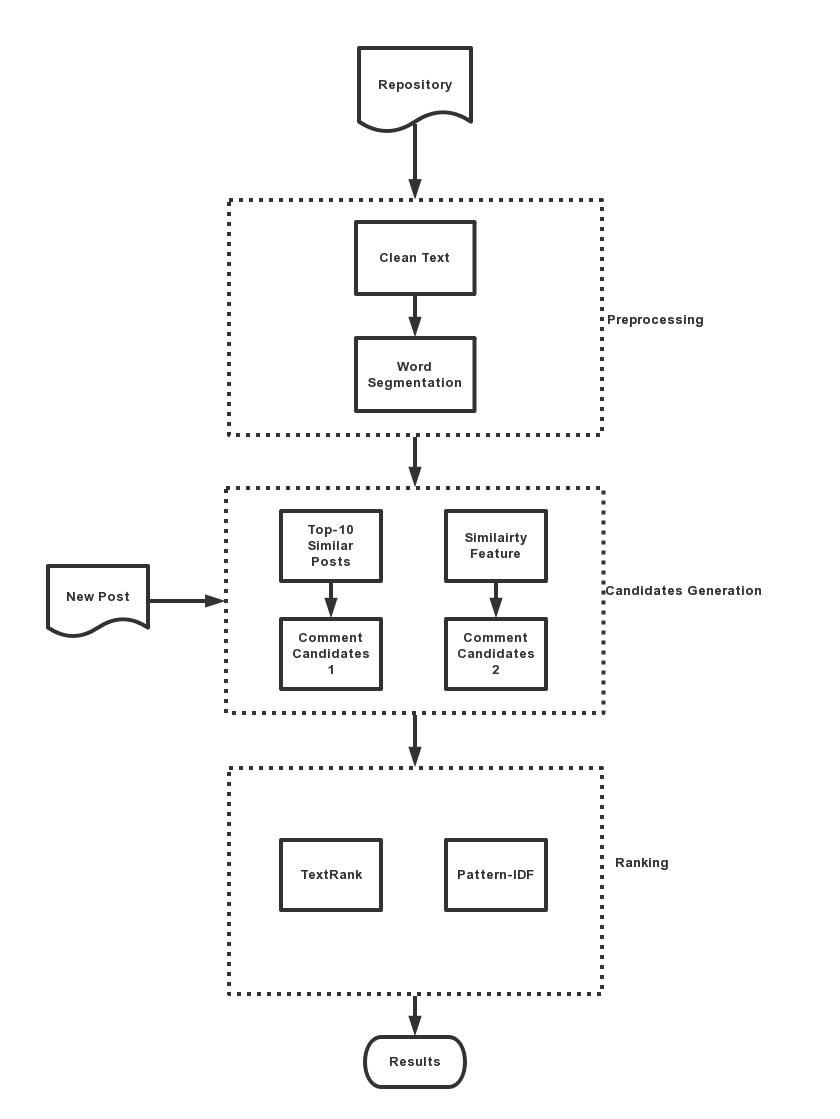
\includegraphics[height=4.6in, width=3.3in]{stc-flow.png}
        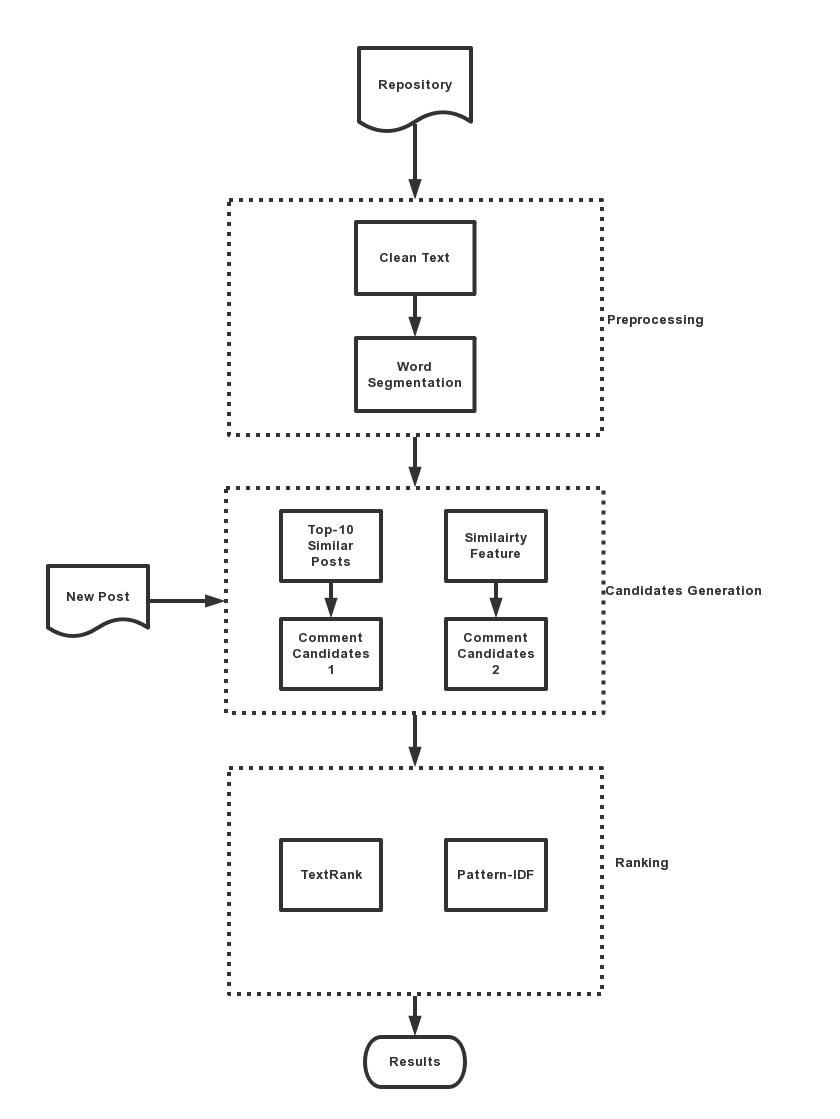
\includegraphics{stc-flow.png}
    \end{tikzfigure}
    
  }

  \makeatletter
  \newcounter{tablecounter}
  \newenvironment{tikztable}[1][]{
    \def \rememberparameter{#1}
    \vspace{10pt}
    \refstepcounter{tablecounter}
    \begin{center}
    }{
      \ifx\rememberparameter\@empty
      \else
      \\[10pt]
      {\small Tab.~\thetablecounter: \rememberparameter}
      \fi
    \end{center}
  }
  \makeatother

  \startsecondcolumn 

  \blocknode{Result}%
  {
    \begin{tikzfigure}[The official results of five runs for Nders team]
      \begin{tabular}{lccc}
      \hline
       Run        &  Mean nG@1  &  Mean P+  &  Mean nERR@10  \\ \hline
       Nders-C-R1 & 0.4593 & 0.5394 & 0.5805 \\ %\hline
       Nders-C-R2 & 0.4743 & \textbf{0.5497} & \textbf{0.5882} \\ %\hline
       Nders-C-R3 & 0.4647 & 0.5317 & 0.5768 \\ %\hline
       Nders-C-R4 & \textbf{0.4780} & 0.5338 & 0.5809 \\ %\hline
       Nders-C-R5 & 0.4550 & 0.5495 & 0.5868 \\ \hline
      \end{tabular}
    \end{tikzfigure}
    
  }


  \blocknode{Conclusions}%
  {
    In this paper, we propose an approach for STC-2 task of NTCIR-13. The LSA,
Word2Vec and LSTM-Sen2Vec model are used to find similar posts. The LSA and Word2Vec 
model are used to retrieve comment candidates. A graph-based algorithm TextRank 
and the Pattern-IDF we devised are applied to rank the candidates. Results show 
that the Pattern-IDF we devised is effective for ranking while TextRank not, 
and LDA model outperforms LSA model in retrieving candidates. Finally, our best 
run achieves 0.4780(R4) for mean nG@1, 0.5497(R2) for mean P+, and 0.5882(R2) for 
mean nERR@10, which respectively rankes 4th, 5th, 5th among 22 teams. 
    
  }
  
  \blocknode{Acknowledgements}%
  {
    Thanks for ...
  }
  



\end{tikzpicture}


\end{document}




